\documentclass[11pt,a4paper]{article}

% ------------------------------------------------------------
% Pacotes
% ------------------------------------------------------------
\usepackage[utf8]{inputenc}
\usepackage[T1]{fontenc}
\usepackage[portuguese]{babel}
\usepackage{lmodern}
\usepackage[a4paper,margin=2.5cm]{geometry}
\usepackage{graphicx}
\usepackage{float}
\usepackage{booktabs}
\usepackage{tabularx}
\usepackage{array}
\usepackage{amsmath}
\usepackage{xcolor}
\usepackage{listings}
\usepackage{caption}
\usepackage{enumitem}
\usepackage{tikz}
\usepackage[hidelinks]{hyperref}

\definecolor{verdeUA}{RGB}{87,176,38}

\setlength{\parskip}{0.5em}
\setlength{\parindent}{0pt}
\setlist{itemsep=0.2em}

% ------------------------------------------------------------
% Listagens de código MATLAB
% ------------------------------------------------------------
\definecolor{codebg}{RGB}{248,248,248}
\definecolor{codecomment}{RGB}{34,139,34}
\definecolor{codekeyword}{RGB}{0,0,180}
\definecolor{codestring}{RGB}{160,32,240}

\lstdefinestyle{matlab}{
  language=Matlab,
  basicstyle=\ttfamily\footnotesize,
  keywordstyle=\color{codekeyword}\bfseries,
  commentstyle=\color{codecomment},
  stringstyle=\color{codestring},
  backgroundcolor=\color{codebg},
  numbers=left,
  numberstyle=\tiny\color{gray},
  numbersep=6pt,
  frame=single,
  rulecolor=\color{gray!40},
  breaklines=true,
  breakatwhitespace=false,
  showstringspaces=false,
  tabsize=4,
  columns=fullflexible,
  keepspaces=true,
  literate=
    {á}{{\'a}}1 {à}{{\`a}}1 {â}{{\^a}}1 {ã}{{\~a}}1
    {é}{{\'e}}1 {ê}{{\^e}}1 {í}{{\'i}}1
    {ó}{{\'o}}1 {ô}{{\^o}}1 {õ}{{\~o}}1 {ú}{{\'u}}1
    {ç}{{\c{c}}}1 {Á}{{\'A}}1 {É}{{\'E}}1 {Í}{{\'I}}1
    {Ó}{{\'O}}1 {Ú}{{\'U}}1 {Ç}{{\c{C}}}1 {Ã}{{\~A}}1
    {º}{{\textordmasculine}}1 {ª}{{\textordfeminine}}1
}
\lstset{style=matlab}

% Atalhos
\newcommand{\code}[1]{\texttt{#1}}

% ------------------------------------------------------------
\begin{document}

% ============================================================
% CAPA
% ============================================================
\begin{titlepage}
  \begin{tikzpicture}[remember picture, overlay]
    \draw[verdeUA, line width=10pt]
      ([xshift=1.5cm, yshift=-1.5cm]current page.north west)
      rectangle
      ([xshift=-1.5cm, yshift=1.5cm]current page.south east);
  \end{tikzpicture}

  \centering
  \vspace*{0.3cm}
  \IfFileExists{logo_ua.png}{%
    
\includegraphics[width=0.5\textwidth]{logo_ua.png}%
  }{%
    \fbox{\parbox[c][2.5cm][c]{0.5\textwidth}{\centering UA logo}}%
  }\par

  \vfill
  {\color{verdeUA}\rule{\linewidth}{1.2pt}}\par
  \vspace{0.5cm}
  {\Huge\scshape Avaliação de Desempenho de\\[0.3cm]
   Ligações Ponto-a-Ponto com\\[0.3cm]
   Múltiplos Fluxos de Pacotes\par}
  \vspace{0.5cm}
  {\color{verdeUA}\rule{\linewidth}{1.2pt}}\par
  \vspace{0.8cm}

  {\Large\scshape\color{verdeUA} Mini-Projeto 1\par}
  \vspace{0.3cm}
  {\large Modelação e Desempenho de Redes e Serviços \textperiodcentered{} Ano Letivo 2026/2027\par}

  \vfill
  {\large\textbf{Grupo}\par}
  \vspace{0.3cm}
  {\large José Fernandes -- 114472 \hspace{1.8cm}}\\
   Pedro Venda -- 139321\par}

  \vspace{0.6cm}
  {\large\textbf{Autoavaliação da percentagem de trabalho}\par}
  \vspace{0.3cm}
  {\large José Fernandes -- 50\%\\
   Pedro Venda -- 50\%\par}

  \vspace{0.8cm}
  {\large\textbf{Docente}\par}
  \vspace{0.3cm}
  {\large Prof. Amaro de Sousa\par}

  \vfill
  {\large Departamento de Eletrónica, Telecomunicações e Informática\\
   Universidade de Aveiro\par}
  \vspace{0.6cm}
  {\large Novembro de 2026\par}
  \vspace*{0.3cm}
\end{titlepage}

\tableofcontents
\newpage

% ============================================================
% 1. INTRODUÇÃO
% ============================================================
\section{Introdução}

Neste mini-projeto estudámos o desempenho de uma ligação de $C = 10$ Mbps que suporta 3 fluxos de pacotes. Usámos simulação de eventos discretos e modelos teóricos, e comparámos três algoritmos de escalonamento.

\begin{itemize}
  \item \textbf{Task 1 -- FIFO:} uma única fila para todos os fluxos, validada com o modelo M/G/1;
  \item \textbf{Task 2 -- Priority Queuing (PQ):} o Fluxo 3 tem a prioridade mais alta, validada com o modelo M/G/1 com prioridades;
  \item \textbf{Task 3 -- Deficit Round Robin (DRR):} uma fila por fluxo, validada com o princípio de \textit{max-min fairness} ponderado.
\end{itemize}


% \subsection{Fluxos e casos de tráfego}

% Os tamanhos dos pacotes de cada fluxo têm todos a mesma probabilidade (Tabela~\ref{tab:fluxos}). O tempo de transmissão de um pacote de $B$ Bytes é $S = 8B/C$.

% \begin{table}[H]
% \centering
% \caption{Características dos fluxos.}
% \label{tab:fluxos}
% \begin{tabular}{cccc}
% \toprule
% Fluxo & Tamanhos (Bytes) & Tamanho médio $E[B]$ & $E[S] = 8E[B]/C$ \\
% \midrule
% 1 & 100 -- 1500 & 800 B & 0,640 ms \\
% 2 & 100 -- 150  & 125 B & 0,100 ms \\
% 3 & 500 -- 1000 & 750 B & 0,600 ms \\
% \bottomrule
% \end{tabular}
% \end{table}

% \begin{table}[H]
% \centering
% \caption{Casos de tráfego e carga da ligação $\rho = \sum_i \lambda_i E[S_i]$.}
% \label{tab:casos}
% \begin{tabular}{ccccc}
% \toprule
% Caso & $\lambda_1$ (pps) & $\lambda_2$ (pps) & $\lambda_3$ (pps) & $\rho$ \\
% \midrule
% A & 400  & 400  & 600  & 0,656 \\
% B & 600  & 600  & 600  & 0,804 \\
% C & 800  & 800  & 600  & 0,952 \\
% D & 1000 & 1000 & 1000 & 1,340 (congestionado) \\
% \bottomrule
% \end{tabular}
% \end{table}

% \subsection{Metodologia}

% Em todas as experiências corremos $N = 50$ simulações, cada uma com o critério de paragem $P = 100\,000$ pacotes transmitidos. Para cada parâmetro de desempenho apresentamos a média das 50 simulações e o intervalo de confiança a 90\%:
% \begin{equation}
% \bar{X}(N) \pm z_{1-\alpha/2}\sqrt{\frac{S^2(N)}{N}}, \qquad \alpha = 0{,}1, \quad z_{0{,}95} = 1{,}6449
% \end{equation}

% Os parâmetros estimados para cada fluxo são: a perda de pacotes PL (\%), o atraso médio APD (ms), o atraso máximo MPD (ms) e o \textit{throughput} transmitido TT (Mbps).

% Nos gráficos, as barras são a média e as barras de erro são o intervalo de confiança.

% Cada exercício é composto por um script (\code{MiniProject\_ExN\_Jose\_Fernandes\_Pedro\_Venda.m}) e o respetivo simulador. Colocamos o código completo no Anexo~\ref{sec:anexo}.

% ============================================================
% 2. TASK 1
% ============================================================
% \newpage
\section{Task 1 -- FIFO}

\subsection{1.a -- Simulador \code{Sim2FlowsMP}}

\begin{table}[H]
\centering
\caption{Alterações do \code{Sim2Flows} para o \code{Sim2FlowsMP}.}
\label{tab:alt1}
\begin{tabularx}{\textwidth}{c X c c}
\toprule
\# & Alteração & Linhas (original) & Linhas (nova) \\
\midrule
1  & Novo parâmetro de entrada \code{flows} (tamanhos de cada fluxo) & 1 & 1, 7 \\
2  & \code{FLOW\_NUM = length(flows)} & -- & 14 \\
3  & Fila pré-alocada com $P$ posições e contador \code{queue\_count} & 19--20 & 22--27 \\
4  & Contadores estatísticos com uma posição por fluxo & 23--28 & 30--35 \\
5  & Primeira chegada de cada fluxo criada num ciclo & 40--44 & 47--54 \\
6  & Próximo evento escolhido com \code{min} em vez de \code{sortrows} & 48--54 & 66--73 \\
7  & Tamanho do próximo pacote gerado a partir do seu fluxo & 59--63 & 79 \\
8  & Chegada: pacote colocado na fila pré-alocada & 69--74 & 85--92 \\
9  & Partida: pacote retirado da fila pré-alocada & 83--92 & 101--114 \\
10 & Gerador de tamanhos genérico \code{GenerateSize(flow)} & 104--120 & 126--128 \\
\bottomrule
\end{tabularx}
\end{table}

\textbf{Justificação das principais alterações:}
\begin{itemize}
  \item \textbf{Parâmetro \code{flows} e \code{FLOW\_NUM} (1, 2, 4):} no original, os tamanhos estavam escritos dentro do simulador e só davam para 2 fluxos. Passámos a usar os tamanhos como argumento (\code{flows = \{100:1500; 100:150; 500:1000\}}); assim, o simulador funciona para qualquer número de fluxos e os contadores ficam com uma posição por fluxo. Isto foi feito para caso fosse necessário alguma alteração futura e para melhor percebermos o conceito do programa, já que nos obriga a entender quais são as variáveis que necessitam de mudança e o porquê.
  \item \textbf{Primeira chegada (5):} o original só criava as chegadas dos fluxos 1 e 2; alterámos para que o Fluxo 3 passasse também a ter pacotes.
  \item \textbf{Tamanho do pacote e gerador (7, 10):} o \code{if/else} só distinguia 2 fluxos e as distribuições eram as do exemplo das aulas. Como no enunciado todos os tamanhos têm igual probabilidade, alterámos para \code{randi([min max])}.
  \item \textbf{Otimizações (3, 6, 8, 9):} passámos a usar \code{min} em vez de ordenar a lista de eventos e a pré-alocar a fila, o que evita copiar matrizes em cada iteração.
  Passámos de 3,5s por simulação para cerca de 1,3s, o que nos permitiu passar mais tempo a desenvolver e menos a testar.
\end{itemize}

\begin{lstlisting}
FLOW_NUM = length(flows);
...
QUEUE = zeros(P,3);
queue_count = 0;     % Tracks current number of packets in queue
...
EventList = zeros(FLOW_NUM, 5);
for k = 1:FLOW_NUM
    tmp = Clock + exprnd(1/lambda(k));
    EventList(k,:) = [ARRIVAL, tmp, GenerateSize(flows{k}), k, tmp];
end
...
% more optimization processes the sortrows takes a looong time
    [~, idx] = min(EventList(:,2));
    Event      = EventList(idx, 1);
    Clock      = EventList(idx, 2);
    PacketSize = EventList(idx, 3);
    Flow       = EventList(idx, 4);
    ArrInstant = EventList(idx, 5);
    EventList(idx, :) = [];
    
    switch Event
        case ARRIVAL         % If event is an ARRIVAL
            ...
            if STATE==0
               ...
            else
                if QUEUEOCCUPATION + PacketSize <= f
                    queue_count = queue_count + 1;
                    QUEUE(queue_count, :) = [PacketSize , Clock, Flow];
                    QUEUEOCCUPATION= QUEUEOCCUPATION + PacketSize;
                ...
            end
        case DEPARTURE          % If event is a DEPARTURE
            ...
            if QUEUEOCCUPATION > 0
                QSize= QUEUE(1,1);
                QInstant= QUEUE(1,2);
                QFlow= QUEUE(1,3);
                EventList = [EventList; DEPARTURE, Clock + 8*QSize/(C*1e6), QSize, QFlow, QInstant];
                QUEUEOCCUPATION= QUEUEOCCUPATION - QSize;
                if queue_count > 1
                    QUEUE(1:queue_count-1, :) = QUEUE(2:queue_count, :);
                end
                queue_count = queue_count - 1;
                ...

function out= GenerateSize(flow)
    out= randi([flow(1) flow(length(flow))]);
end
\end{lstlisting}

\subsection{1.b -- Simulação do caso C}

Na alínea b obtivemos os seguintes resultados.

\begin{figure}[H]
\centering
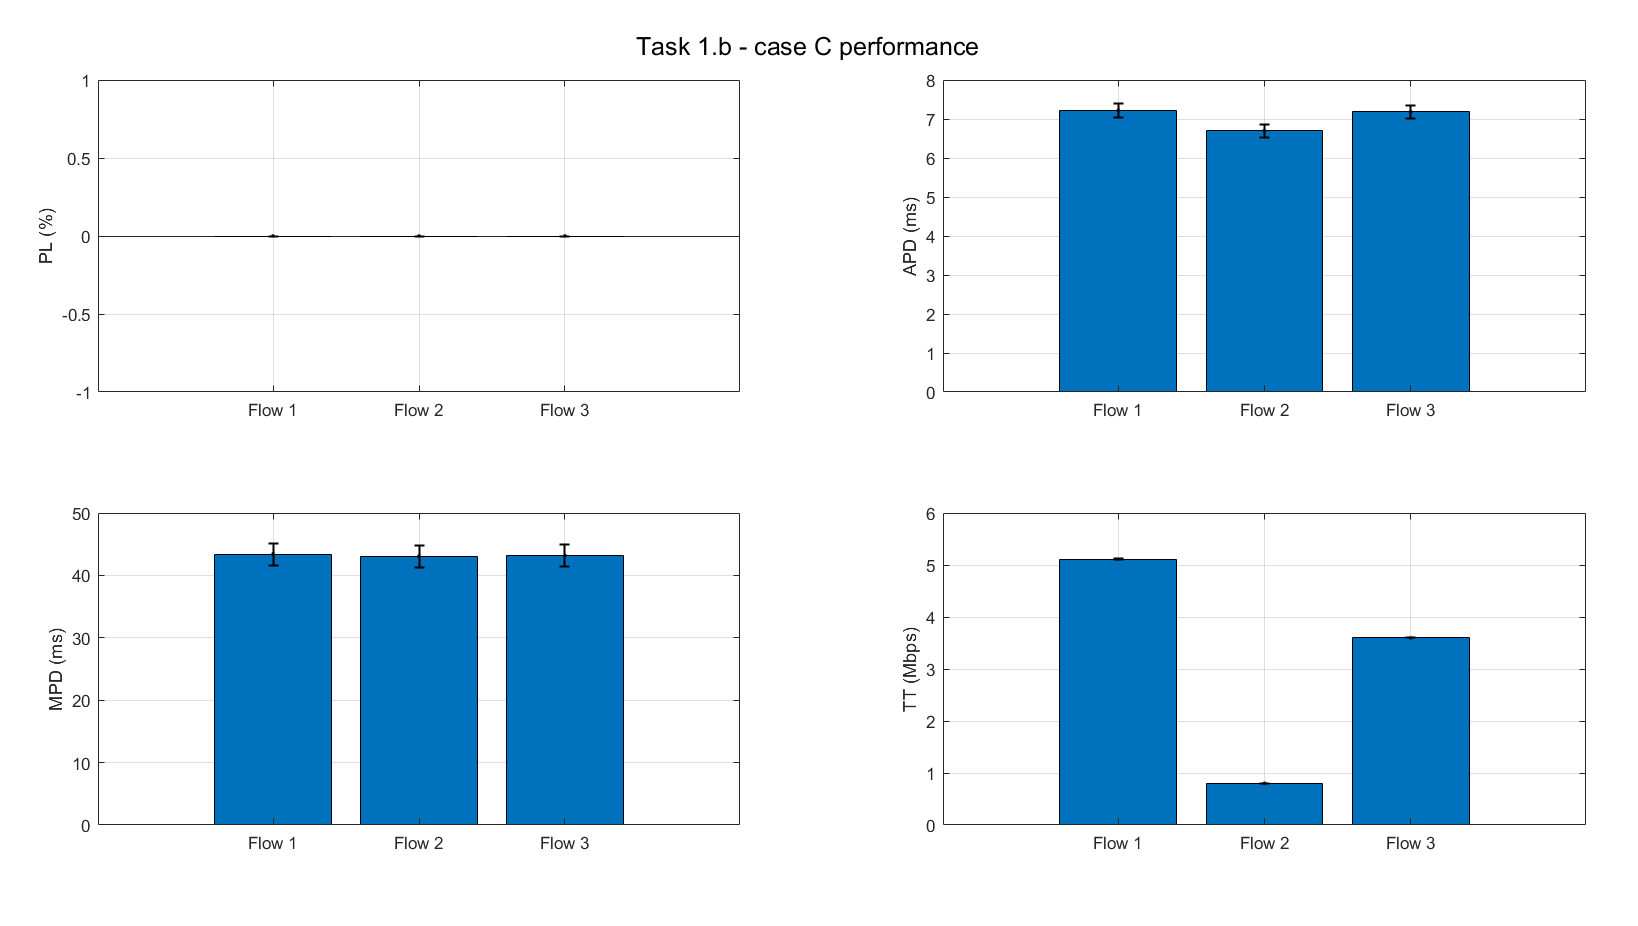
\includegraphics[width=1\textwidth]{figures/Task1b.png}
\caption{Task 1.b -- FIFO, caso C.}
\end{figure}

\begin{table}[H]
\centering
\caption{Resultados da 1.b (média $\pm$ IC 90\%).}
\begin{tabular}{lccc}
\toprule
Parâmetro & Fluxo 1 & Fluxo 2 & Fluxo 3 \\
\midrule
PL (\%)   & 0 & 0 & 0 \\
APD (ms)  & 7,10 $\pm$ 0,13 & 6,56 $\pm$ 0,12 & 7,05 $\pm$ 0,12 \\
MPD (ms)  & 42,2 $\pm$ 1,5 & 41,8 $\pm$ 1,6 & 42,1 $\pm$ 1,6 \\
TT (Mbps) & 5,115 $\pm$ 0,007 & 0,800 $\pm$ 0,001 & 3,596 $\pm$ 0,005 \\
\bottomrule
\end{tabular}
\end{table}

\textbf{Justificações e Conclusões:}
\begin{itemize}
  \item \textbf{Não há perdas:} Devido ao tamanho de 1\,MB, a fila nunca chega a encher e não existem perdas.
  \item \textbf{O \textit{throughput} de cada fluxo é igual ao débito que chega} ($\lambda_i \cdot 8 \cdot E[B_i]$ = 5,12, 0,80 e 3,60 Mbps), porque todos os pacotes são transmitidos.
  \item \textbf{Os atrasos máximos são praticamente iguais:} como o sistema implementado é FIFO e os três fluxos partilham a mesma fila, têm atrasos máximos iguais, pois este sistema não favorece nenhum dos fluxos.
  \item \textbf{Average packet delay desigual:} Apesar da fila FIFO não priveligiar nenhum dos fluxos, o que faz com que o seu tempo médio em fila seja igual, como a variável considera também o tempo de transmissão, o fluxo com o menor average packet (Fluxo 2) é ligeiramente mais rápido.
\end{itemize}

\subsection{1.c -- Modelo M/G/1}

A fórmula teórica para cada fluxo foi calculada da seguinte maneira (esta demonstração foi simplicada e não contém os cálculos de todos os fluxos):
\begin{lstlisting}
Es_f1  = sum(p_flow1.*(8*flow1/C_bps));
Es2_f1 = sum(p_flow1.*(8*flow1/C_bps).^2);

rho1 = lambda1(3) * Es_f1;
rho_total = rho1 + rho2 + rho3;

Wq = (lambda1(3)*Es2_f1 + lambda2(3)*Es2_f2 + lambda3(3)*Es2_f3)/(2 * (1 - rho_total));
%a posição 3 do lambda indica a ordem dos casos 3->C
W1 = Wq + Es_f1;

avg_B_f1 = sum(flow1)/numel(flow1);
throughput_f1 = lambda1(3)*(8*avg_B_f1);
\end{lstlisting}

E foram obtidos os seguintes resultados:
\begin{figure}[H]
\centering
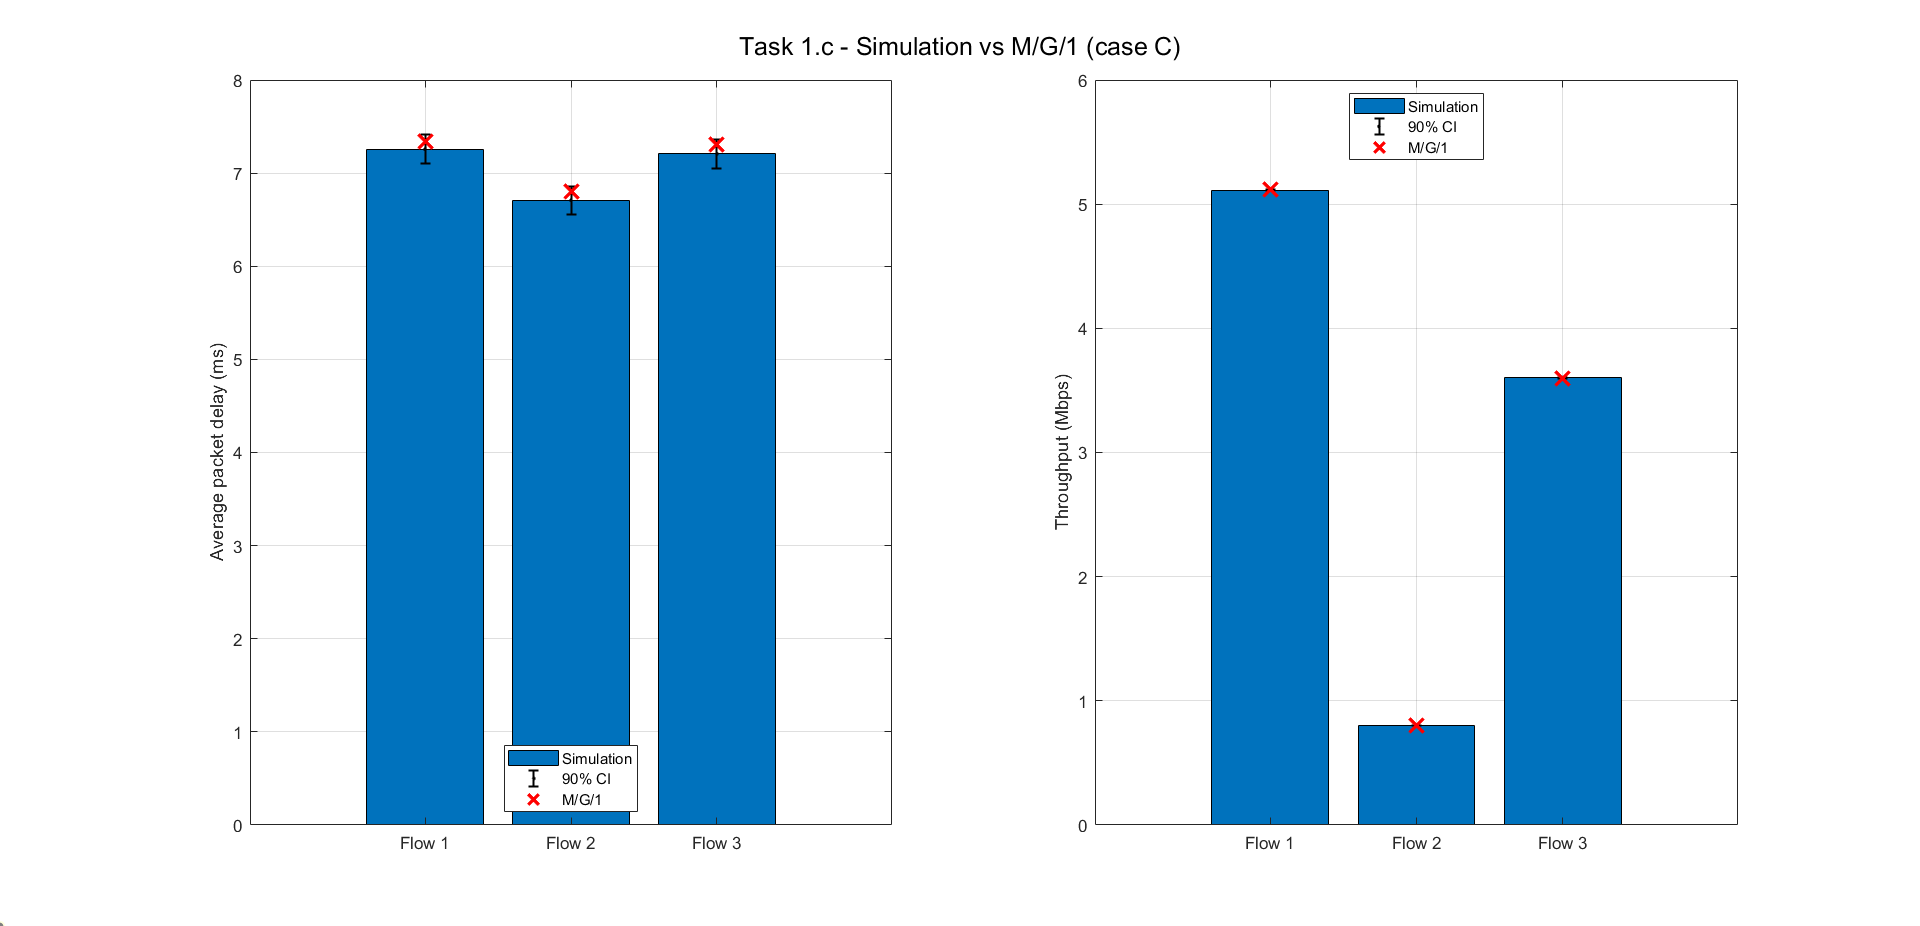
\includegraphics[width=1\textwidth]{figures/Task1c.png}
\caption{Task 1.c -- Simulação vs M/G/1 (caso C).}
\end{figure}

\begin{table}[H]
\centering
\caption{Comparação entre a teoria (M/G/1) e a simulação (1.b).}
\begin{tabular}{lccc}
\toprule
 & Fluxo 1 & Fluxo 2 & Fluxo 3 \\
\midrule
APD -- M/G/1 (ms)     & 7,344 & 6,804 & 7,304 \\
APD -- simulação (ms) & 7,099 $\pm$ 0,126 & 6,555 $\pm$ 0,123 & 7,048 $\pm$ 0,124 \\
Diferença relativa    & $-3{,}3\%$ & $-3{,}7\%$ & $-3{,}5\%$ \\
\midrule
TT -- M/G/1 (Mbps)     & 5,120 & 0,800 & 3,600 \\
TT -- simulação (Mbps) & 5,115 $\pm$ 0,007 & 0,800 $\pm$ 0,001 & 3,596 $\pm$ 0,005 \\
\bottomrule
\end{tabular}
\end{table}

\textbf{Conclusões:}
\begin{itemize}
  \item O atraso simulado fica cerca de 3,5\% abaixo do teórico. Com a ligação quase cheia ($\rho \approx 0{,}95$) o atraso varia muito entre simulações.
\end{itemize}

\subsection{1.d -- Fluxo 3 nos casos A, B e C}

\begin{figure}[H]
\centering
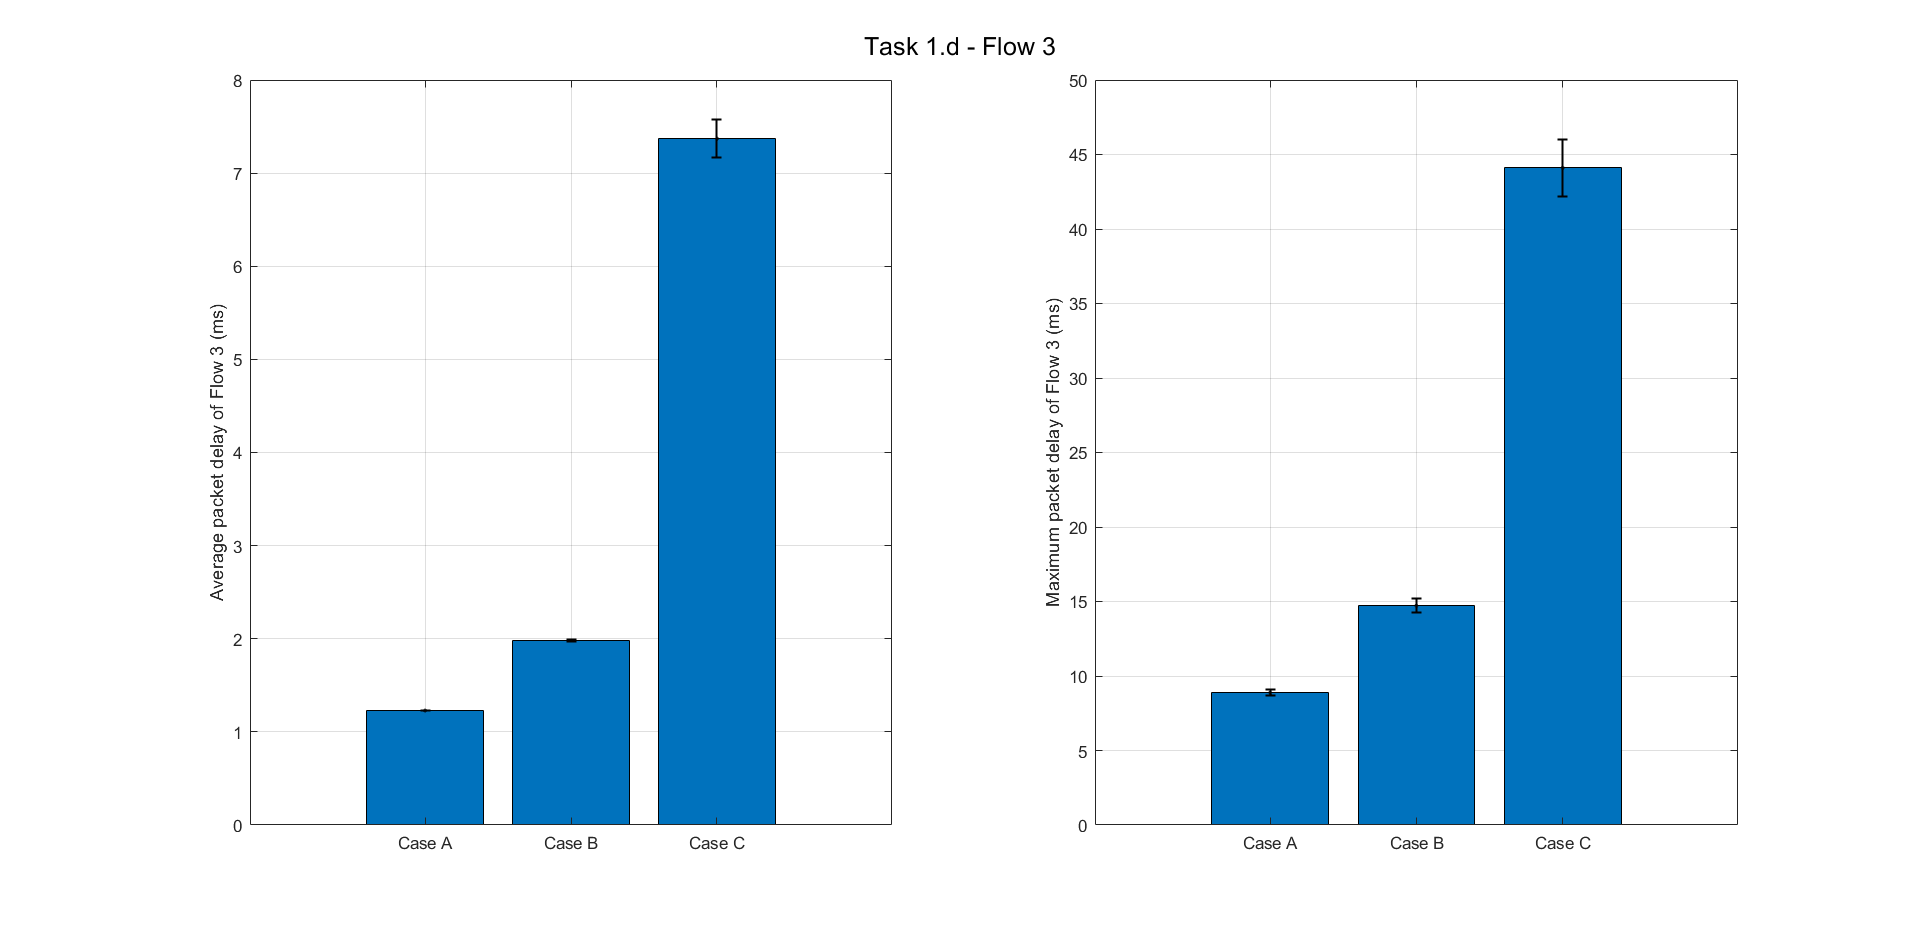
\includegraphics[width=1\textwidth]{figures/Task1d.png}
\caption{Task 1.d -- atraso médio e máximo do Fluxo 3 com FIFO.}
\end{figure}

\begin{table}[H]
\centering
\caption{Fluxo 3 com FIFO nos casos A, B e C.}
\begin{tabular}{ccccc}
\toprule
Caso & $\rho$ & APD (sim.) & APD (M/G/1) & MPD (sim.) \\
\midrule
A & 0,656 & 1,231 $\pm$ 0,003 ms & 1,231 ms & 9,07 $\pm$ 0,26 ms \\
B & 0,804 & 1,981 $\pm$ 0,009 ms & 1,974 ms & 14,9 $\pm$ 0,4 ms \\
C & 0,952 & 7,38 $\pm$ 0,20 ms   & 7,30 ms  & 43,7 $\pm$ 2,2 ms \\
\bottomrule
\end{tabular}
\end{table}

\vspace{1em}
\vspace{1em}
\vspace{2em} 
\noindent\textbf{Justificações e conclusões:}
\begin{itemize}
  \item Apesar da taxa de chegada do fluxo 3 ser constante, o seu atraso fica 6 vezes maior de A para C. Isto acontece, porque a taxa de utilização do link dos outros fluxos aumenta. 
  \item O atraso dispara perto de $\rho = 1$.
\end{itemize}
% ============================================================
% 3. TASK 2
% ============================================================
% \newpage
\section{Task 2 -- Priority Queuing}

\subsection{2.a -- Simulador \code{Sim2FlowsPrioMP}}

% O enunciado pede uma nova versão do \code{Sim2FlowsPrio}. 

Partimos do nosso \code{Sim2FlowsMP} (Task 1), que já suporta 3 fluxos e as otimizações descritas na secção anterior, e acrescentámos o que é preciso para ter prioridades: o Fluxo 3 tem a prioridade mais alta e os Fluxos 1 e 2 a segunda.

\begin{table}[H]
\centering
\caption{Alterações do \code{Sim2FlowsMP} para o \code{Sim2FlowsPrioMP}.}
\begin{tabularx}{\textwidth}{c X c c}
\toprule
\# & Alteração & Linhas (\code{Sim2FlowsMP}) & Linhas (nova) \\
\midrule
1 & Novo parâmetro \code{prio}; \code{f} passa a vetor (um tamanho por fila) & 1--7 & 1--8 \\
2 & \code{PRIO\_NUM = max(prio)} & -- & 16 \\
3 & Uma fila por prioridade (cell array \code{QUEUE\{q\}}) & 22--27 & 24--31 \\
4 & Chegada: pacote vai para a fila da sua prioridade & 85--92 & 72--80 \\
5 & Partida: próximo pacote sai da fila de prioridade mais alta não vazia & 101--114 & 89--103 \\
\bottomrule
\end{tabularx}
\end{table}

\textbf{Justificação das principais alterações:}
\begin{itemize}
  \item \textbf{Parâmetros \code{prio} e \code{f} (1, 2):} no \code{Sim2FlowsMP} havia uma só fila, com um único tamanho \code{f}, e nenhum fluxo tinha prioridade. Passámos a usar o vetor \code{prio} como argumento no caso (\code{prio = [2 2 1]}, com o Fluxo 3 na fila 1) e o \code{f} passou a vetor, com um tamanho por fila assim as prioridades e os tamanhos das filas mudam sem mexer no simulador.
  \item \textbf{Uma fila por prioridade (3):} no \code{Sim2FlowsMP} todos os pacotes iam para a mesma fila. Como o PQ precisava de uma fila por prioridade, alterámos para um \textit{cell array}: \code{QUEUE\{1\}} é a fila do Fluxo 3 e \code{QUEUE\{2\}} as dos Fluxos 1 e 2, cada uma com a sua ocupação e o seu contador.
  \item \textbf{Chegada (4):} antes, o pacote entrava na fila única e perdia-se se essa fila estivesse cheia. Alterámos para que o pacote só ocupe espaço na fila da sua prioridade e só se perca se essa fila estiver cheia.
  \item \textbf{Partida (5):} antes, saía sempre o primeiro pacote da fila única. Passámos a escolher o pacote da fila de prioridade mais alta que não estivesse vazia: um pacote dos Fluxos 1 ou 2 só é transmitido quando não houver pacotes do Fluxo 3 à espera, e dentro de cada fila a ordem continua a ser FIFO.
\end{itemize}
% \pagebreak


Código da secção 2.a:

\begin{lstlisting}[firstnumber=72]
                % fila da prioridade do pacote
                q = prio(Flow);
                if QUEUEOCCUPATION(q) + PacketSize <= f(q)
                    queue_count(q) = queue_count(q) + 1;
                    QUEUE{q}(queue_count(q), :) = [PacketSize , Clock, Flow];
                    QUEUEOCCUPATION(q)= QUEUEOCCUPATION(q) + PacketSize;
                else
                    LOSTPACKETS(Flow)= LOSTPACKETS(Flow) + 1;
                end
...
            % fila de prioridade mais alta não vazia
            q = find(queue_count > 0, 1);
            if ~isempty(q)
                QSize= QUEUE{q}(1,1);
\end{lstlisting}

\subsection{2.b -- Simulação do caso C}

\begin{figure}[H]
\centering
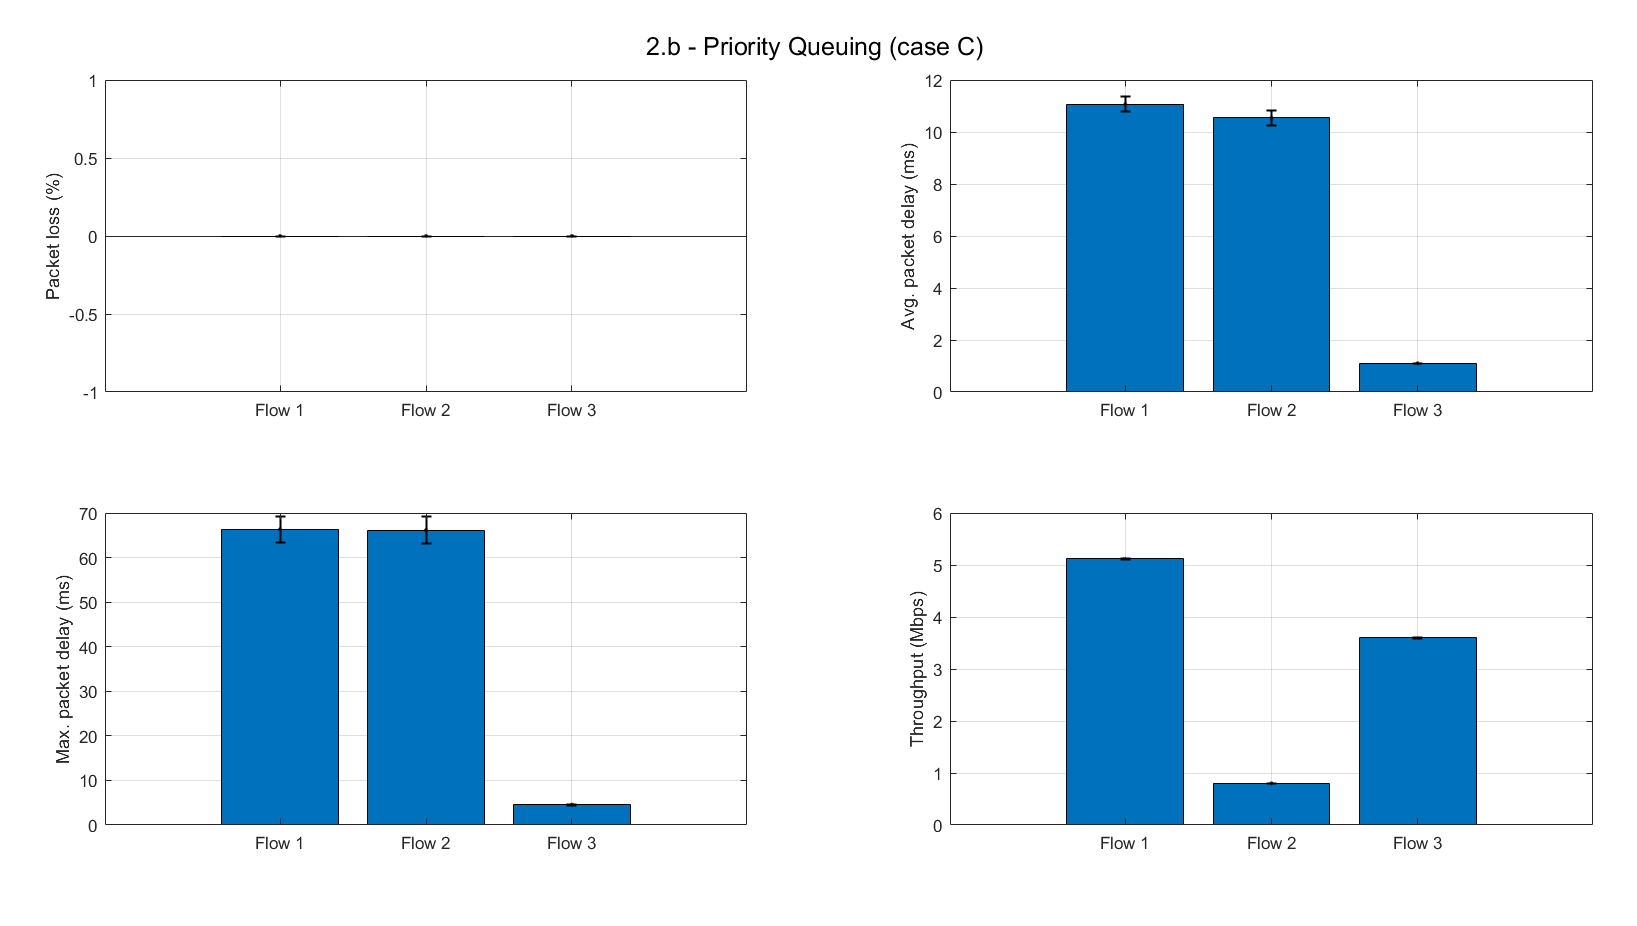
\includegraphics[width=1\textwidth]{figures/Task2b.png}
\caption{Task 2.b -- Priority Queuing caso C.}
\end{figure}

\begin{table}[H]
\centering
\caption{Resultados da 2.b (média $\pm$ IC 90\%).}
\begin{tabular}{lccc}
\toprule
Parâmetro & Fluxo 1 & Fluxo 2 & Fluxo 3 \\
\midrule
PL (\%)   & 0 & 0 & 0 \\
APD (ms)  & 10,74 $\pm$ 0,25 & 10,20 $\pm$ 0,25 & 1,101 $\pm$ 0,002 \\
MPD (ms)  & 67,0 $\pm$ 3,1 & 66,9 $\pm$ 3,1 & 4,48 $\pm$ 0,09 \\
TT (Mbps) & 5,114 $\pm$ 0,007 & 0,800 $\pm$ 0,001 & 3,596 $\pm$ 0,005 \\
\bottomrule
\end{tabular}
\end{table}

\vspace{4em}

\textbf{Justificação entre fluxos:}
\begin{itemize}
  \item O Fluxo 3 passa à frente dos outros devido a sua prioridade, por isso tem atrasos muito baixos (1,1 ms em média).
  \item Os Fluxos 1 e 2 partilham a fila de prioridade baixa e ficam com atrasos semelhantes (cerca de 10--11 ms).
  \item Perdas e \textit{throughput} iguais aos da 1.b: as prioridades só mudam a ordem de transmissão.
\end{itemize}

\textbf{Comparação com a 1.b (FIFO):}

\begin{table}[H]
\centering
\caption{Atrasos com FIFO (1.b) e com prioridades (2.b).}
\begin{tabular}{lccc}
\toprule
 & Fluxo 1 & Fluxo 2 & Fluxo 3 \\
\midrule
APD FIFO (ms) & 7,10 & 6,56 & 7,05 \\
APD PQ (ms)   & 10,74 & 10,20 & 1,10 \\
\midrule
MPD FIFO (ms) & 42,2 & 41,8 & 42,1 \\
MPD PQ (ms)   & 67,0 & 66,9 & 4,48 \\
\bottomrule
\end{tabular}
\end{table}

\begin{itemize}
  \item O Fluxo 3 ganha cerca de 6 ms no atraso médio; 
  \item os Fluxos 1 e 2 perdem cerca de 3,6 ms. Uma vez que O PQ não reduz o atraso total, só o redistribui entre fluxos.
\end{itemize}

\subsection{2.c -- Modelo M/G/1 com prioridades}

Primeiro calculámos o tempo médio de transmissão de cada fluxo e a parte da ligação que cada um ocupa: o Fluxo 3, com prioridade alta, ocupa 36\% da ligação, e os Fluxos 1 e 2, com prioridade baixa, ocupam 59,2\%. Depois calculámos o tempo de espera na fila de cada prioridade:
\begin{itemize}
  \item \textbf{Prioridade alta (Fluxo 3):} só espera que acabe o pacote que está a ser transmitido e pelos outros pacotes do Fluxo 3, por isso o tempo na fila depende só da carga do próprio Fluxo 3.
  \item \textbf{Prioridade baixa (Fluxos 1 e 2):} espera também por todos os pacotes do Fluxo 3, por isso o tempo na fila depende da carga total da ligação e fica muito maior.
\end{itemize}
Por fim, o atraso de cada fluxo é o tempo na fila da sua prioridade mais o tempo de transmissão do próprio pacote.

\vspace{1em}
Código da secção 2.c:

\begin{lstlisting}
rho = v_lambda_C.*ES;                        % ocupação de cada fluxo
num = sum(v_lambda_C.*ES2);                  % soma de todos os fluxos
rho_alta = sum(rho(prio==1));                % prioridade 1: fluxo 3
rho_baixa = sum(rho(prio==2));               % prioridade 2: fluxos 1 e 2
WQ_alta = num/(2*(1-rho_alta));                          % fila prioridade alta
WQ_baixa = num/(2*(1-rho_alta)*(1-rho_alta-rho_baixa));  % fila prioridade baixa
WQ = zeros(1,3);
WQ(prio==1) = WQ_alta;
WQ(prio==2) = WQ_baixa;
theory_packet_delay = (WQ + ES)*1000;        % fila + transmissão (ms)
\end{lstlisting}

\begin{figure}[H]
\centering
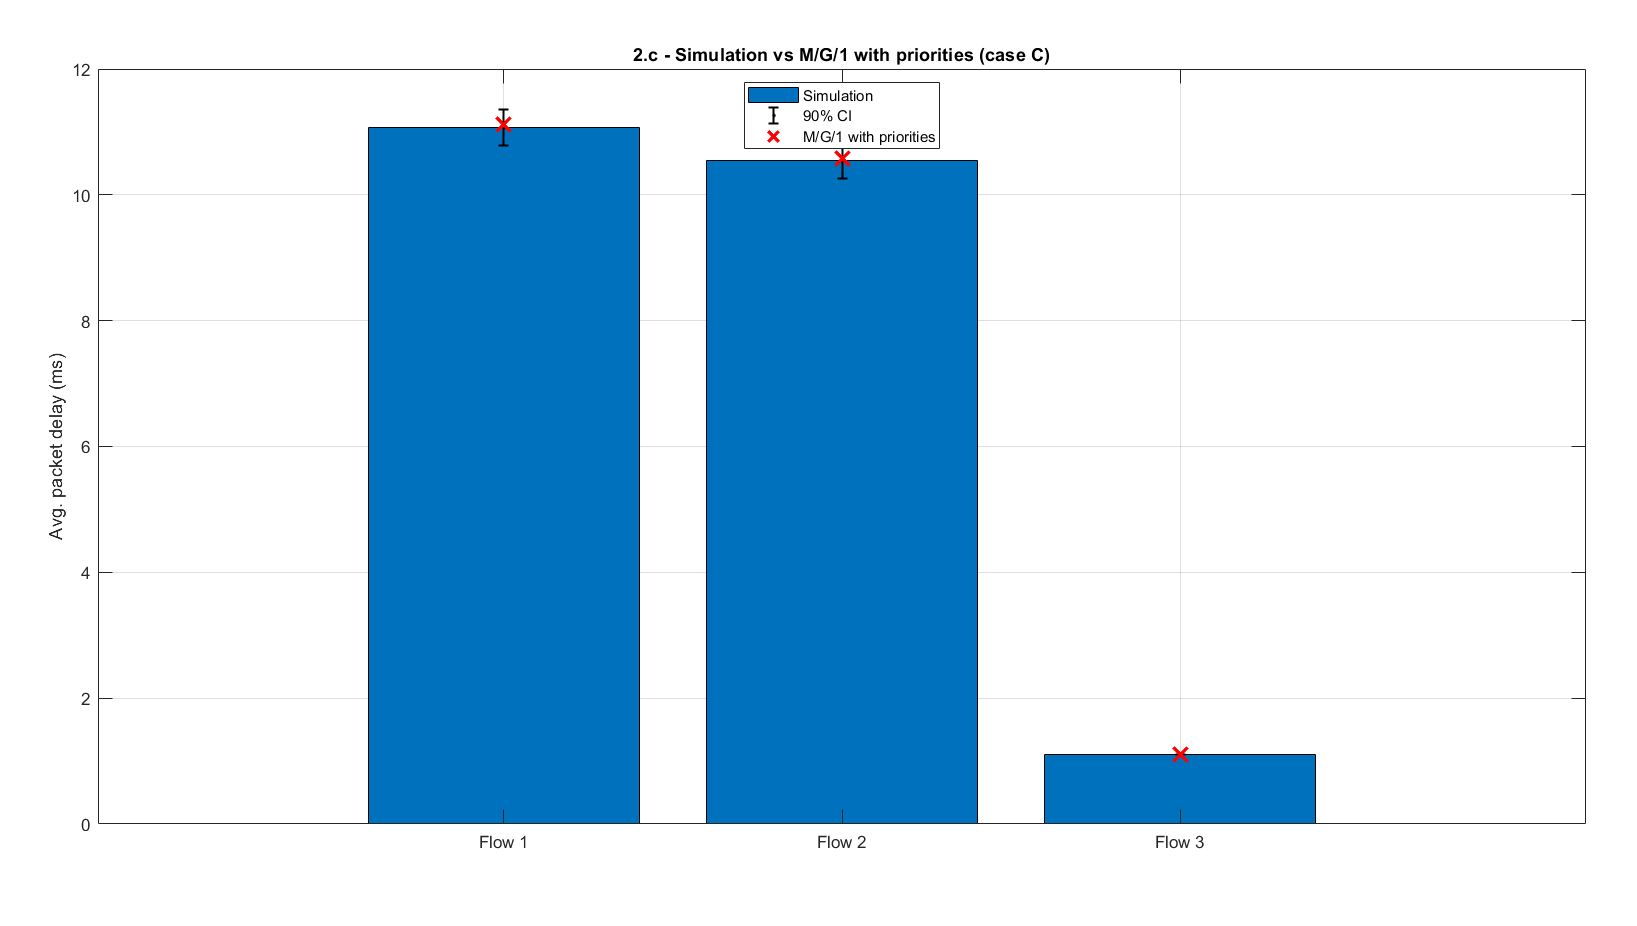
\includegraphics[width=1\textwidth]{figures/Task2c.png}
\caption{Task 2.c -- Simulação vs M/G/1 com prioridades (caso C).}
\end{figure}

\begin{table}[H]
\centering
\caption{Comparação entre a teoria e a simulação (2.b).}
\begin{tabular}{lccc}
\toprule
APD (ms) & Fluxo 1 & Fluxo 2 & Fluxo 3 \\
\midrule
M/G/1 com prioridades & 11,115 & 10,575 & 1,103 \\
Simulação (2.b)       & 11,075 $\pm$ 0,285 & 10,535 $\pm$ 0,275 & 1,102 $\pm$ 0,002 \\
Diferença relativa    & $-0{,}4\%$ & $-0{,}4\%$ & $-0{,}1\%$ \\
\bottomrule
\end{tabular}
\end{table}

\textbf{Conclusões:}
\begin{itemize}
  \item Tal como esperado, todos os valores teóricos coincidem dentro da faixa de erro das simulações.
  \item Nos fluxos 1 e 2 a simulação fica cerca de 0.4\% abaixo, uma vez que "absorvem" um maior impacto da saturação do link, por terem menor prioridade.
\end{itemize}

\subsection{2.d -- Fluxo 3 nos casos A, B e C}

\begin{figure}[H]
\centering
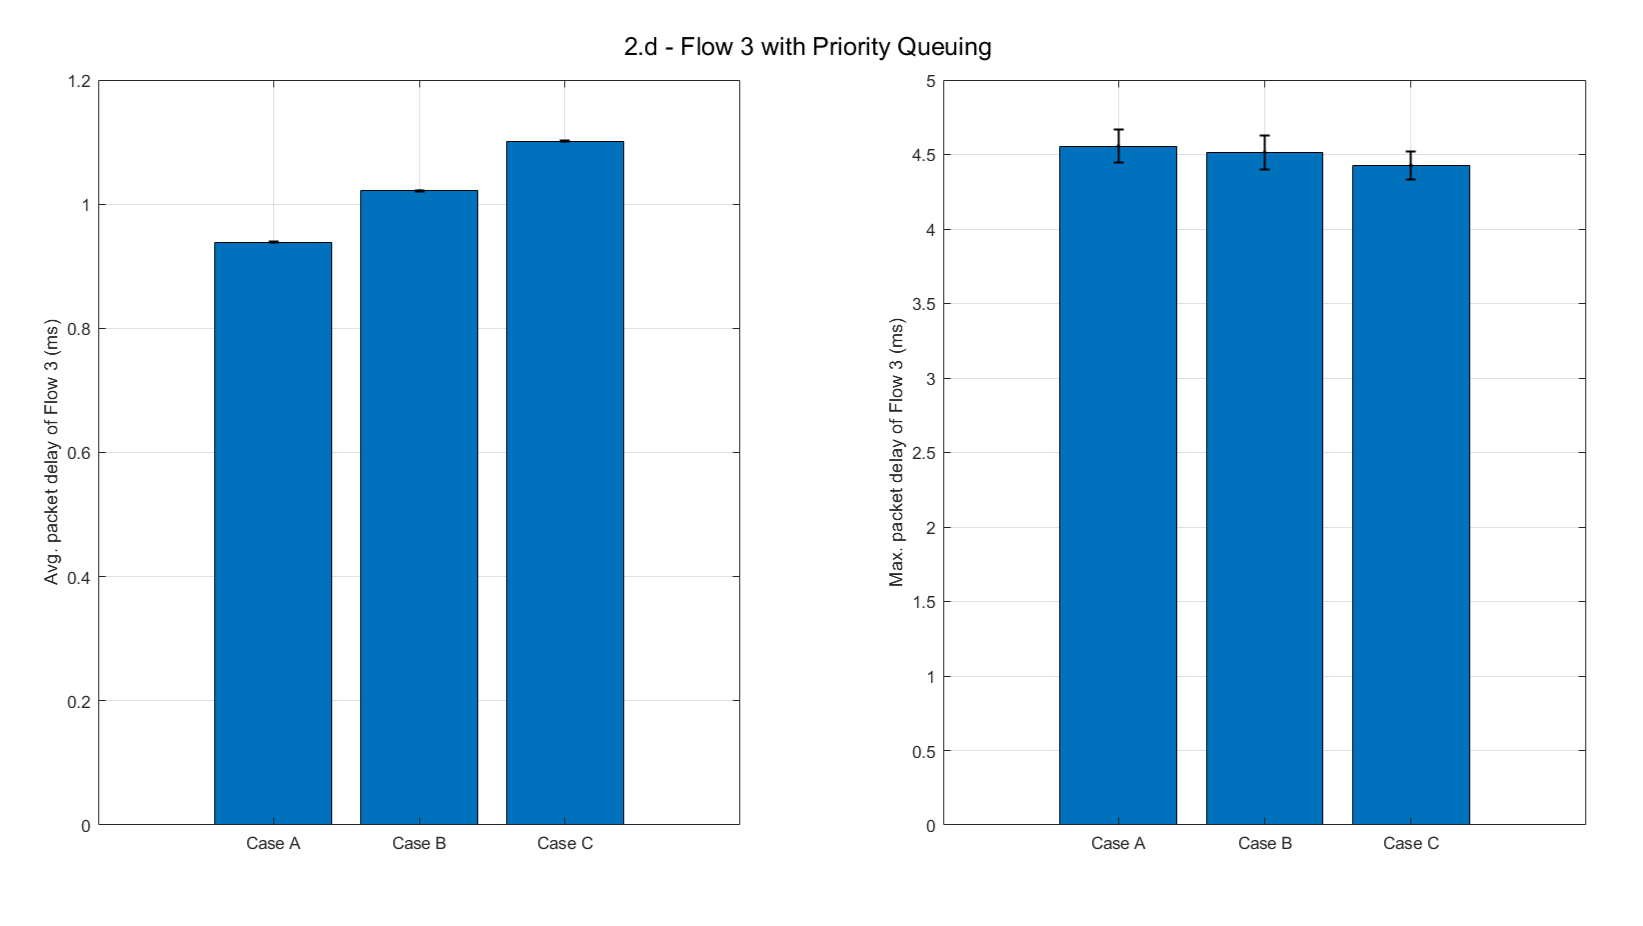
\includegraphics[width=1\textwidth]{figures/Task2d.png}
\caption{Task 2.d -- Fluxo 3 com prioridades}
\end{figure}

\begin{table}[H]
\centering
\caption{Fluxo 3: FIFO (1.d) vs prioridades (2.d).}
\begin{tabular}{ccccccc}
\toprule
Caso & $\rho$ & APD FIFO & APD PQ & APD PQ (teoria) & MPD FIFO & MPD PQ \\
\midrule
A & 0,656 & 1,231 ms & 0,938 ms & 0,939 ms & 9,07 ms & 4,47 ms \\
B & 0,804 & 1,981 ms & 1,021 ms & 1,021 ms & 14,9 ms & 4,46 ms \\
C & 0,952 & 7,38 ms  & 1,102 ms & 1,103 ms & 43,7 ms & 4,40 ms \\
\bottomrule
\end{tabular}
\end{table}

\textbf{Justificações, comparação com a 1.d e conclusões:}
\begin{itemize}
    \item Existe um pequeno aumento do \textit{avg. packet delay} do caso A para o C, porque como o tráfego dos flows 1 e 2 aumenta, cresce a probabilidade de estar ocupado com um pacote de baixa prioridade;
    \item Com PQ, o atraso do Fluxo 3 quase não muda de A para C (0,94 $\rightarrow$ 1,10 ms) e o máximo fica nos 4,5 ms. 
  Com FIFO, este quase que crescia 6 vezes. Isto acontece, pois a prioridade faz com que o fluxo deixe de ser afetado pelo congestionamento do link;
    \item Apesar do gráfico não o demonstrar, é importante ter em consideração que para o bom funcionamento do fluxo 3 com a PQ, os restantes fluxos de menor prioridade são altamente prejudicados. O mesmo não acontece com o FIFO.
\end{itemize}

% ============================================================
% 4. TASK 3
% ============================================================
\newpage
\section{Task 3 -- Deficit Round Robin}

\subsection{3.a -- Simulador \code{Sim2FlowsDRRMP}}

Partimos também do nosso primeiro Simulador \code{Sim2FlowsMP} e acrescentámos o DRR: uma fila por fluxo e, em cada ronda, uma vez que os fluxos são servidos pela ordem do ID (1, 2, 3).

\begin{table}[H]
\centering
\caption{Alterações do \code{Sim2FlowsMP} para o \code{Sim2FlowsDRRMP}.}
\begin{tabularx}{\textwidth}{c X c c}
\toprule
\# & Alteração & Linhas (\code{Sim2FlowsMP}) & Linhas (nova) \\
\midrule
1 & Novo parâmetro \code{Quantum}; \code{f} passa a vetor (uma fila por fluxo) & 1--7 & 1--8 \\
2 & Uma fila por fluxo (cell array \code{QUEUE\{q\}}) & 22--27 & 23--30 \\
3 & Fila final \code{FINALQUEUE} e crédito \code{CREDIT} de cada fluxo & -- & 31--32 \\
4 & Chegada: pacote vai para a fila do seu fluxo & 85--92 & 73--80 \\
5 & Partida: ronda DRR quando a fila final está vazia & -- & 89--115 \\
6 & Próximo pacote a transmitir sai da fila final & 101--114 & 116--125 \\
\bottomrule
\end{tabularx}
\end{table}

\textbf{Justificação das principais alterações:}
\begin{itemize}
  \item \textbf{Parâmetros \code{Quantum} e \code{f} (1):} Desta vez no \code{Sim2FlowsMP} não havia quantum e a fila única tinha de ter só tamanho \code{f}.Decidimos então passar a usar o vetor \code{Quantum} como argumento, com o número de bytes em que cada fluxo pode enviar por ronda, e passamos o \code{f} a vetor, com um tamanho por fila.
  \item \textbf{Filas e variáveis do DRR (2, 3):} no \code{Sim2FlowsMP} todos os pacotes iam para a mesma fila. Como o DRR precisava de uma fila por fluxo, mudamos esta para um \textit{cell array} (\code{QUEUE\{1\}}, \code{QUEUE\{2\}} e \code{QUEUE\{3\}}) e acrescentámos a fila final (\code{FINALQUEUE}), onde ficam os pacotes escolhidos em cada ronda, e o crédito de cada fluxo (\code{CREDIT}), com os bytes que cada um ainda pode enviar.
  \item \textbf{Chegada (4):} antes, o pacote entrava na fila única e perdia-se se essa fila estivesse cheia.
  Neste caso alteramos isso para que o pacote só ocupe espaço na fila do seu fluxo; assim, em caso de congestionamento, quem envia demasiado enche apenas a sua própria fila sem tirar espaço aos outros.
  \item \textbf{Ronda DRR (5):} Passámos a fazer uma ronda sempre que a fila final fica vazia: para cada fluxo com pacotes, somamos o quantum ao respetivo crédito e passamos para a fila final os primeiros pacotes que cabem nesse crédito. O crédito que sobrar ficaria então para a ronda seguinte, e uma fila vazia fica com crédito zero.
  \item \textbf{Transmissão (6):} antes, no nosso simulador este saia sempre o primeiro pacote da fila única. Alterámos este e os pacotes passaram a ser transmitidos a partir da fila final, pela ordem da ronda.
\end{itemize}

\vspace{6em}

\begin{lstlisting}[firstnumber=91]
            while isempty(FINALQUEUE) && any(queue_count > 0)
                for q = 1:FLOW_NUM
                    if queue_count(q) > 0
                        CREDIT(q) = CREDIT(q) + Quantum(q);
                        % move os primeiros pacotes cujo tamanho total nao excede o credito
                        n = 0;
                        while n < queue_count(q) && QUEUE{q}(n+1,1) <= CREDIT(q)
                            n = n + 1;
                            CREDIT(q) = CREDIT(q) - QUEUE{q}(n,1);
                            QUEUEOCCUPATION(q) = QUEUEOCCUPATION(q) - QUEUE{q}(n,1);
                        end
                        if n > 0
                            FINALQUEUE = [FINALQUEUE; QUEUE{q}(1:n,:)];
                            QUEUE{q}(1:queue_count(q)-n, :) = QUEUE{q}(n+1:queue_count(q), :);
                            queue_count(q) = queue_count(q) - n;
                        end
                        % fila que fica vazia perde o credito
                        if queue_count(q) == 0
                            CREDIT(q) = 0;
                        end
                    else
                        CREDIT(q) = 0;   % fila vazia: credito a zero
                    end
                end
            end
\end{lstlisting}

\subsection{3.b -- Caso C com Quantum = 1500 / 1500 / 1500}

\begin{figure}[H]
\centering
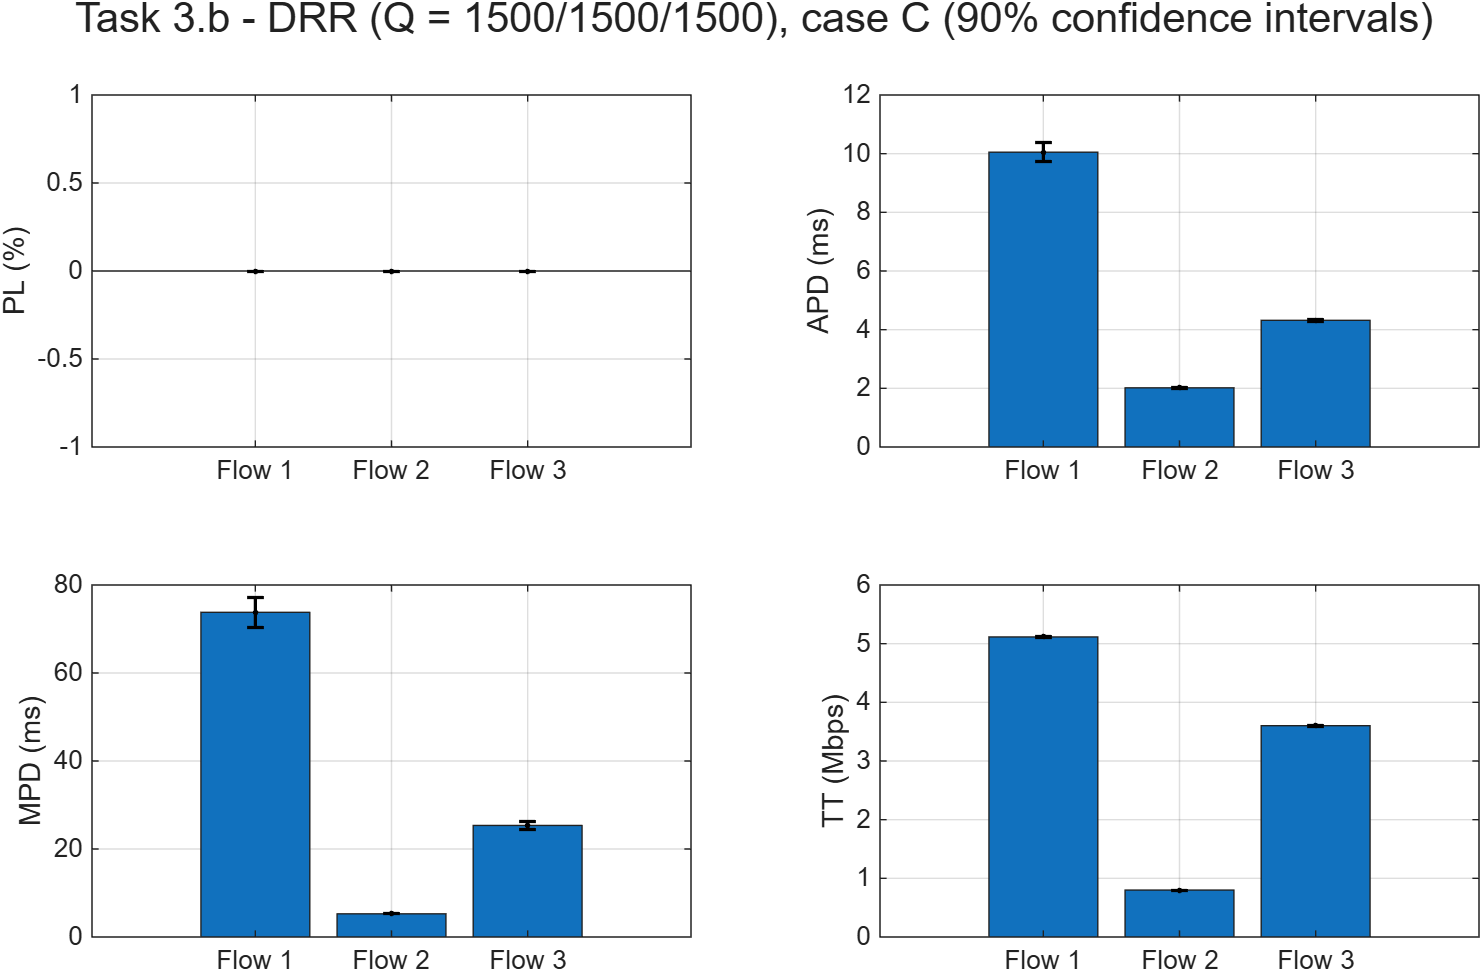
\includegraphics[width=0.9\textwidth]{figures/Task3b.png}
\caption{Task 3.b -- DRR com quanta iguais, caso C.}
\end{figure}

\begin{table}[H]
\centering
\caption{Resultados da 3.b (média $\pm$ IC 90\%).}
\begin{tabular}{lccc}
\toprule
Parâmetro & Fluxo 1 & Fluxo 2 & Fluxo 3 \\
\midrule
PL (\%)   & 0 & 0 & 0 \\
APD (ms)  & 10,05 $\pm$ 0,33 & 2,02 $\pm$ 0,01 & 4,32 $\pm$ 0,04 \\
MPD (ms)  & 73,8 $\pm$ 3,4 & 5,26 $\pm$ 0,03 & 25,4 $\pm$ 0,9 \\
TT (Mbps) & 5,115 $\pm$ 0,008 & 0,800 $\pm$ 0,001 & 3,602 $\pm$ 0,006 \\
\bottomrule
\end{tabular}
\end{table}

\textbf{Justificação entre fluxos:}
\begin{itemize}
  \item Sem perdas e com \textit{throughput} igual ao pedido ($\rho < 1$).
  \item Com quanta iguais, cada fluxo tem direito a cerca de 3,33 Mbps. 
  
  Quem envia menos acaba por esperar menos: 
  Fluxo 2 (0,8 Mbps) 2,0 ms, Fluxo 3 (3,6 Mbps) 4,3 ms, Fluxo 1 (5,12 Mbps) 10 ms.
\end{itemize}

\textbf{Comparação com a 1.b (FIFO) e a 2.b (PQ):}

\begin{table}[H]
\centering
\caption{Atraso médio e máximo no caso C com os três algoritmos.}
\begin{tabular}{lcccccc}
\toprule
 & \multicolumn{3}{c}{APD (ms)} & \multicolumn{3}{c}{MPD (ms)} \\
\cmidrule(lr){2-4}\cmidrule(lr){5-7}
Algoritmo & Fluxo 1 & Fluxo 2 & Fluxo 3 & Fluxo 1 & Fluxo 2 & Fluxo 3 \\
\midrule
FIFO (1.b) & 7,10 & 6,56 & 7,05 & 42,2 & 41,8 & 42,1 \\
PQ (2.b)   & 10,74 & 10,20 & 1,10 & 67,0 & 66,9 & 4,48 \\
DRR (3.b)  & 10,05 & 2,02 & 4,32 & 73,8 & 5,26 & 25,4 \\
\bottomrule
\end{tabular}
\end{table}

\begin{itemize}
  \item FIFO trata todos os fluxos por igual; PQ favorece o Fluxo 3, que tem maior prioridade; e o DRR protege quem envia pouco (Fluxo 2) e penaliza quem envia mais (Fluxo 1).
  \item As Perdas e o \textit{throughput} iguais nos três: só altera quem espera.
\end{itemize}

\subsection{3.c -- Caso D (congestionado) com Quantum = 1500 / 1500 / 1500}

\begin{figure}[H]
\centering
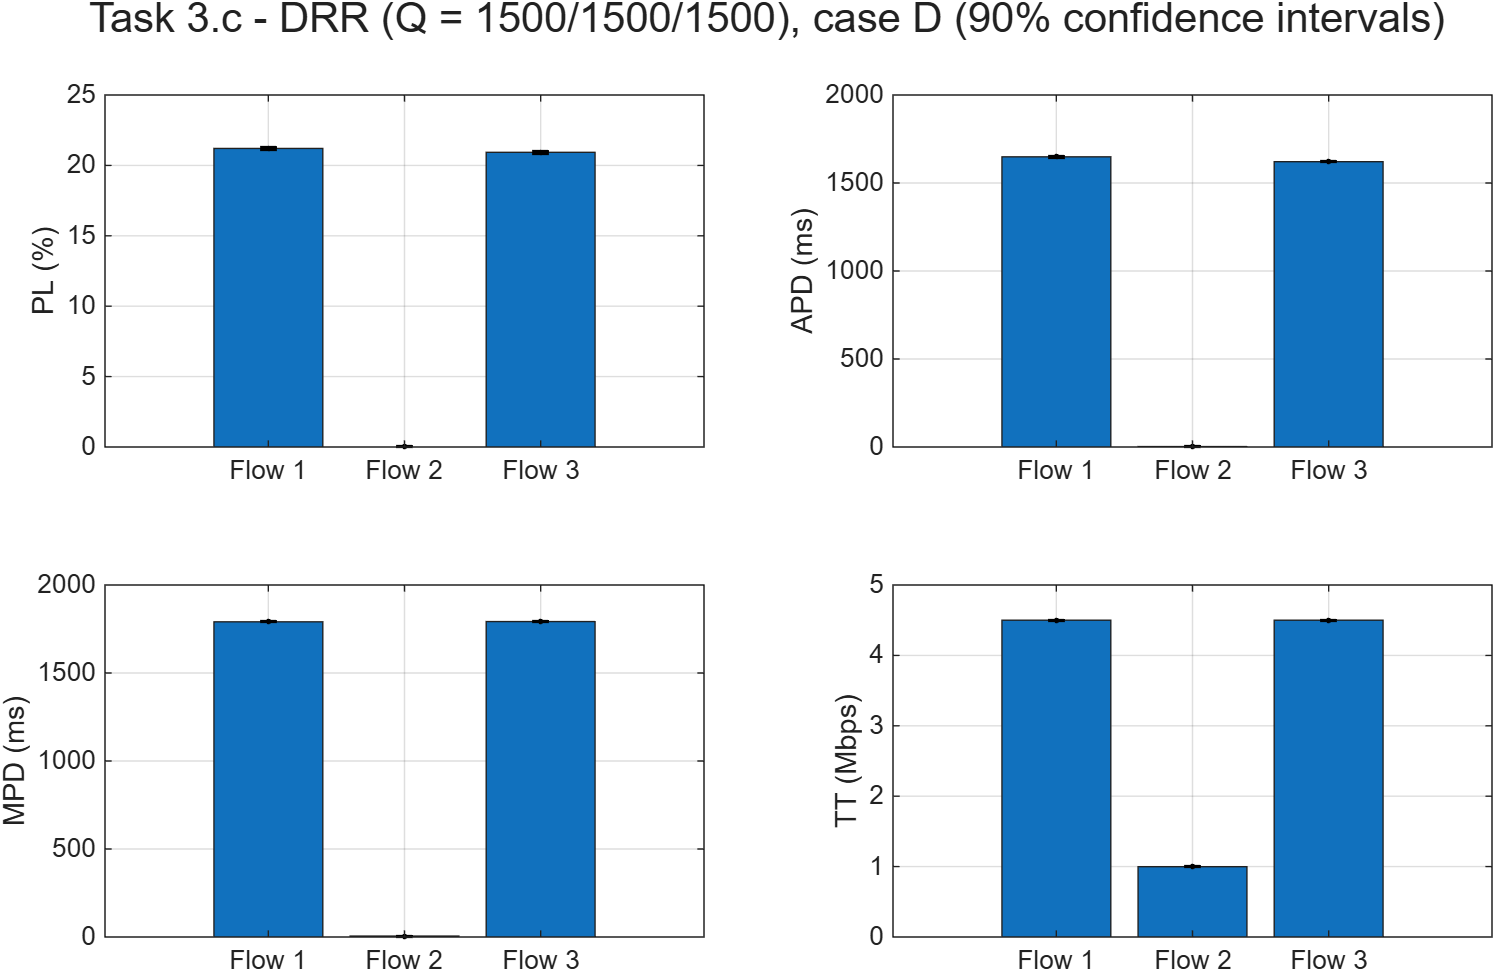
\includegraphics[width=0.9\textwidth]{figures/Task3c.png}
\caption{Task 3.c -- DRR com quanta iguais, caso D.}
\end{figure}

\begin{table}[H]
\centering
\caption{Resultados da 3.c (média $\pm$ IC 90\%).}
\begin{tabular}{lccc}
\toprule
Parâmetro & Fluxo 1 & Fluxo 2 & Fluxo 3 \\
\midrule
PL (\%)   & 21,21 $\pm$ 0,08 & 0 & 20,93 $\pm$ 0,07 \\
APD (ms)  & 1649 $\pm$ 1,4 & 2,79 $\pm$ 0,001 & 1621 $\pm$ 1,4 \\
MPD (ms)  & 1791 $\pm$ 0,7 & 5,50 $\pm$ 0,03 & 1792 $\pm$ 0,7 \\
TT (Mbps) & 4,500 $\pm$ 0,001 & 0,999 $\pm$ 0,001 & 4,500 $\pm$ 0,001 \\
\bottomrule
\end{tabular}
\end{table}

\textbf{Justificação entre fluxos:}
\begin{itemize}
  \item A ligação não chega para tudo (13,4 Mbps pedidos para 10 Mbps). Neste caso o Fluxo 2 pede só 1 Mbps e recebe tudo; os outros dois dividem o resto, 4,5 Mbps cada.
  \item Os Fluxos 1 e 3 enchem as suas filas: perdem cerca de 21\% dos pacotes e esperam cerca de 1,6 s. O Fluxo 2 não perde nada (2,8 ms): o DRR isola os fluxos.
\end{itemize}

\textbf{Comparação com a 3.b:} no caso C o DRR só mudava os atrasos; no caso D este passa a decidir quanto cada fluxo transmite.

\subsection{3.d -- Caso D com Quantum = 1500 / 1500 / 4500}

\begin{figure}[H]
\centering
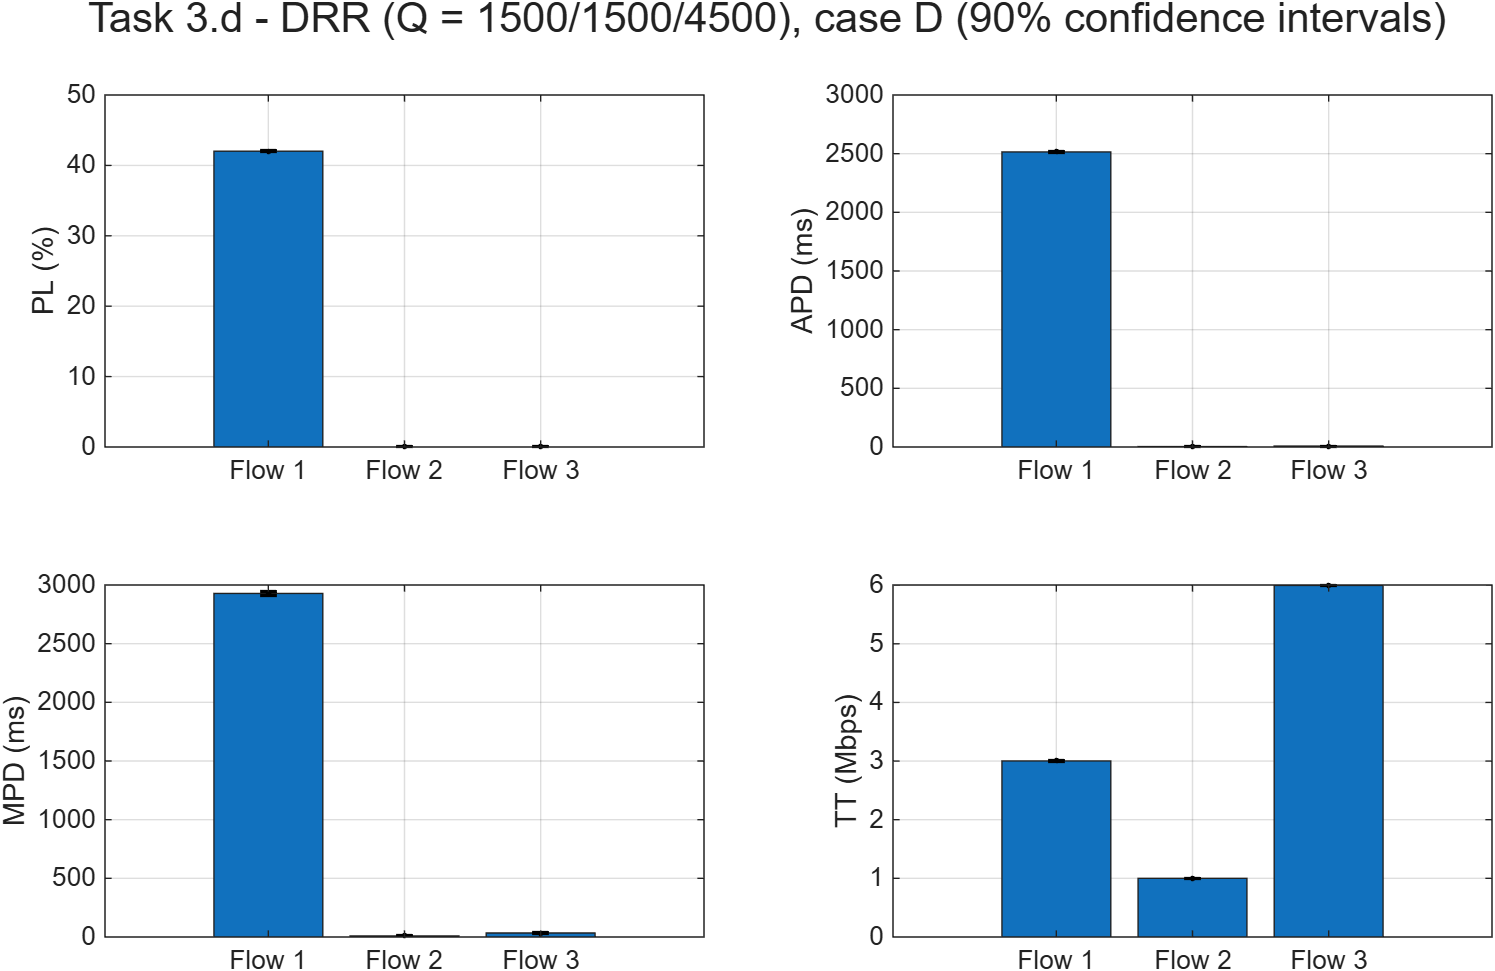
\includegraphics[width=0.9\textwidth]{figures/Task3d.png}
\caption{Task 3.d -- DRR com quanta 1500/1500/4500, caso D.}
\end{figure}

\begin{table}[H]
\centering
\caption{Resultados da 3.d (média $\pm$ IC 90\%).}
\begin{tabular}{lccc}
\toprule
Parâmetro & Fluxo 1 & Fluxo 2 & Fluxo 3 \\
\midrule
PL (\%)   & 42,02 $\pm$ 0,12 & 0 & 0 \\
APD (ms)  & 2514 $\pm$ 6 & 3,72 $\pm$ 0,005 & 7,72 $\pm$ 0,06 \\
MPD (ms)  & 2928 $\pm$ 15 & 9,32 $\pm$ 0,17 & 34,1 $\pm$ 1,4 \\
TT (Mbps) & 3,003 $\pm$ 0,006 & 1,000 $\pm$ 0,001 & 5,997 $\pm$ 0,006 \\
\bottomrule
\end{tabular}
\end{table}

\textbf{Justificação entre fluxos:}
\begin{itemize}
  \item Com o triplo do peso, o Fluxo 3 tem direito a 6 Mbps, exatamente o que pede: sem perdas e com 7,7 ms de atraso.
  \item O Fluxo 2 continua a receber tudo. 
  \item Já Fluxo 1 fica com o que sobra (3 Mbps), perde 42\% dos pacotes e espera cerca de 2,5 s.
\end{itemize}

\textbf{Comparação com a 3.c:}

\begin{table}[H]
\centering
\caption{Caso D com quanta iguais (3.c) e com quanta 1500/1500/4500 (3.d).}
\begin{tabular}{lccc}
\toprule
 & Fluxo 1 & Fluxo 2 & Fluxo 3 \\
\midrule
TT 3.c / 3.d (Mbps)  & 4,50 / 3,00 & 1,00 / 1,00 & 4,50 / 6,00 \\
PL 3.c / 3.d (\%)    & 21,2 / 42,0 & 0 / 0 & 20,9 / 0 \\
APD 3.c / 3.d (ms)   & 1649 / 2514 & 2,8 / 3,7 & 1621 / 7,7 \\
\bottomrule
\end{tabular}
\end{table}


\subsection{3.e -- \textit{Throughput} ideal (\textit{max-min fairness} ponderado)}

No DRR, os pesos do \textit{max-min fairness} são os quanta.
No caso D, os débitos pedidos são $x_i = \lambda_i \cdot 8 \cdot E[B_i]$: $x_1 = 6{,}4$, $x_2 = 1{,}0$ e $x_3 = 6{,}0$ Mbps, com $C = 10$ Mbps.

\textbf{Caso da 3.c -- com pesos 1 : 1 : 1.} Este é ordenando por débito pedido: Fluxo 2 (1,0) < Fluxo 3 (6,0) < Fluxo 1 (6,4).
\begin{enumerate}
  \item Cada fluxo pode receber $d = 10/3 = 3{,}333$ Mbps.
  \item O Fluxo 2 pede $1{,}0 < 3{,}333$ e recebe 1,0 Mbps. Sobram $3{,}333 - 1{,}0 = 2{,}333$ Mbps.
  \item Os outros dois podem receber $d = 3{,}333 + 2{,}333/2 = 4{,}5$ Mbps. Os Fluxos 3 (6,0) e 1 (6,4) pedem mais, por isso recebem \textbf{4,5 Mbps cada}.
\end{enumerate}

\textbf{Caso da 3.d -- com pesos 1 : 1 : 3.} Ordenando pelo débito pedido dividido pelo peso: Fluxo 2 (1,0) < Fluxo 3 (6,0/3 = 2,0) < Fluxo 1 (6,4).
\begin{enumerate}
  \item Repartição inicial proporcional aos pesos: Fluxo 1 $= 10/5 = 2$, Fluxo 2 $= 2$, Fluxo 3 $= 3 \times 10/5 = 6$ Mbps.
  \item O Fluxo 2 pede $1{,}0 < 2$ e recebe 1,0. O Fluxo 3 pede $6{,}0 \le 6$ e recebe 6,0. Sobra $(2-1) + (6-6) = 1$ Mbps.
  \item O Fluxo 1 fica com $2 + 1 = $ \textbf{3,0 Mbps} ($< 6{,}4$).
\end{enumerate}


\begin{lstlisting}
while any(active)
    share = left*weights(w,active)/sum(weights(w,active));
    idx = find(active);
    satisfied = x(idx) <= ideal(idx) + share;
    if ~any(satisfied)
        ideal(idx) = ideal(idx) + share;
        break;
    end
    for j = idx(satisfied)
        left = left - (x(j) - ideal(j));
        ideal(j) = x(j);
        active(j) = false;
    end
end
\end{lstlisting}

\begin{table}[H]
\centering
\caption{\textit{Throughput} ideal vs simulado no caso D (Mbps).}
\begin{tabular}{lccc}
\toprule
 & Fluxo 1 & Fluxo 2 & Fluxo 3 \\
\midrule
3.c -- ideal (1:1:1) & 4,500 & 1,000 & 4,500 \\
3.c -- simulação     & 4,500 $\pm$ 0,001 & 0,999 $\pm$ 0,001 & 4,500 $\pm$ 0,001 \\
\midrule
3.d -- ideal (1:1:3) & 3,000 & 1,000 & 6,000 \\
3.d -- simulação     & 3,003 $\pm$ 0,006 & 1,000 $\pm$ 0,001 & 5,997 $\pm$ 0,006 \\
\bottomrule
\end{tabular}
\end{table}

\textbf{Conclusões:}
\begin{itemize}
  \item A simulação coincide com o \textit{throughput} ideal nos dois casos: o DRR cumpre o \textit{max-min fairness} ponderado, com os quanta como pesos.
\end{itemize}

% ============================================================
% 5. CONCLUSÕES
% ============================================================
% \newpage
% \section{Conclusões gerais}

% \begin{itemize}
%   \item \textbf{FIFO:} simples, mas o atraso de cada fluxo depende do tráfego dos outros.
%   \item \textbf{PQ:} protege o fluxo prioritário (cerca de 1 ms em todos os casos), à custa dos restantes.
%   \item \textbf{DRR:} reparte a ligação de forma justa e, em congestionamento, dá a cada fluxo a parte definida pelos quanta.
%   \item As simulações confirmam os modelos teóricos (M/G/1, M/G/1 com prioridades e \textit{max-min fairness}).
% \end{itemize}

% ============================================================
% ANEXOS
% ============================================================
% \newpage
% \appendix
% \section{Código MATLAB}
% \label{sec:anexo}

% \subsection{Task 2 -- \code{Sim2FlowsPrioMP.m}}
% \lstinputlisting{code/Sim2FlowsPrioMP.m}

% \subsection{Task 2 -- script}
% \lstinputlisting{code/MiniProject_Ex2_Jose_Fernandes_Pedro_Venda.m}

% \subsection{Task 3 -- \code{Sim2FlowsDRRMP.m}}
% \lstinputlisting{code/Sim2FlowsDRRMP.m}

% \subsection{Task 3 -- script}
% \lstinputlisting{code/MiniProject_Ex3_Jose_Fernandes_Pedro_Venda.m}

\end{document}
